\chapter{Metodologi Penelitian}

Bab ini menjelaskan metodologi yang digunakan untuk menyusun karakterisasi spatiotemporal pergerakan kendaraan pada koridor Ring Road Utara. Alur penelitian secara keseluruhan ditunjukkan pada Gambar \ref{fig:pipeline}.

\section{Alur Penelitian}

\begin{figure}[htbp]
\centering
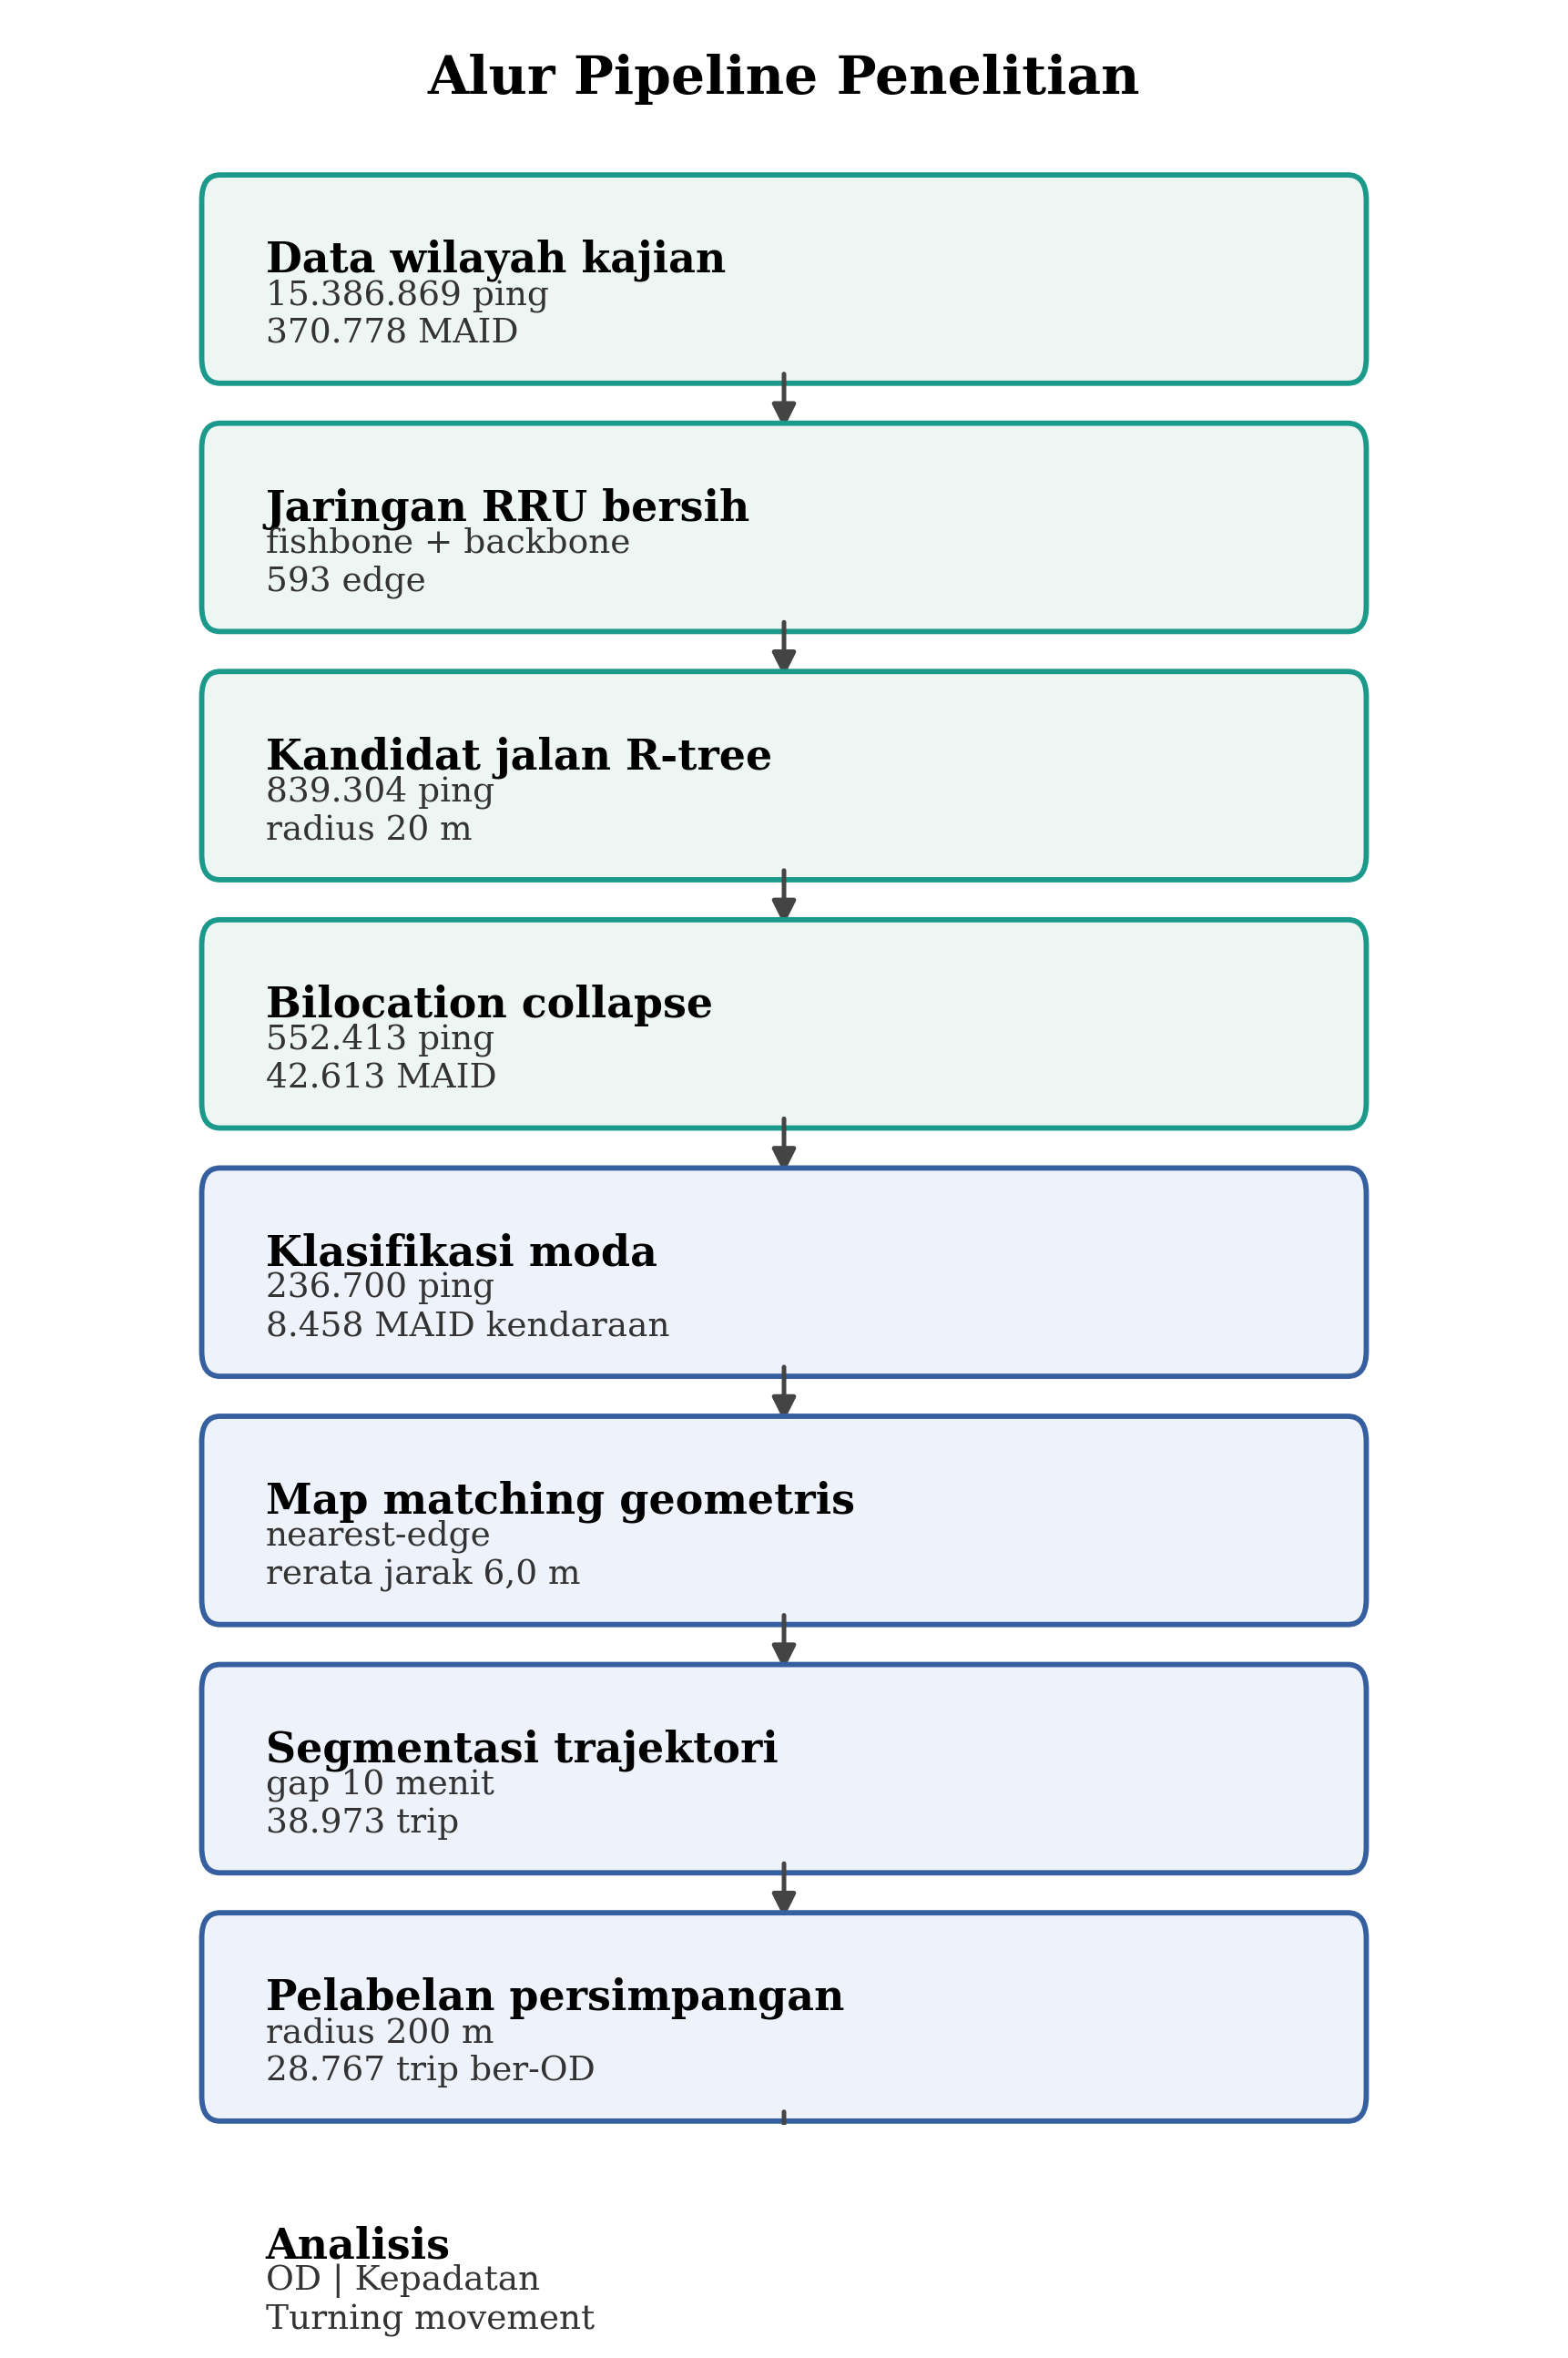
\includegraphics[width=0.95\textwidth]{../results/figures/pipeline/research_pipeline.png}
\caption{Alur pipeline penelitian dari data wilayah kajian hingga analisis OD, intensitas persimpangan, dan pola OD zona eksploratif}
\label{fig:pipeline}
\end{figure}

\section{Data Penelitian}

\subsection{Sumber Data}

Data penelitian berupa MPD aktif yang diperoleh dari kerja sama tim riset dengan salah satu perusahaan telekomunikasi di Indonesia. Dataset mencakup data GPS pada wilayah Daerah Istimewa Yogyakarta dalam periode Oktober 2021 hingga Juni 2022. Setiap observasi terdiri dari identitas perangkat anonim (MAID), koordinat lintang, koordinat bujur, dan waktu pencuplikan.

\subsection{Spesifikasi Data}

Dataset kerja awal yang digunakan dalam pipeline adalah data hasil ekstraksi wilayah kajian Ring Road Utara (\texttt{output\_bbox.parquet}) yang terdiri dari 15.386.869 titik GPS dari 370.778 MAID unik. Setelah penyaringan spasial terhadap jaringan RRU menggunakan R-tree, \textit{bilocation collapse}, dan klasifikasi moda kendaraan bermotor, diperoleh 236.700 titik GPS dari 8.458 MAID yang menunjukkan indikasi kendaraan bermotor pada koridor RRU. Setelah segmentasi trajektori, dataset analisis trip valid terdiri dari 212.407 ping, 8.382 MAID, dan 38.973 trip.

\subsection{Jaringan Jalan}

Jaringan jalan Ring Road Utara dimodelkan menggunakan berkas jaringan bersih hasil kurasi QGIS pada direktori \texttt{data/processed/network}. Jaringan ini digunakan sebagai masukan utama untuk penyaringan spasial, \textit{map matching}, dan pelabelan enam zona persimpangan. Enam zona tersebut adalah Kronggahan, Jombor, Monjali, Kentungan, Condongcatur, dan UPN.

Pada pipeline terbaru, seluruh analisis utama menggunakan basis data yang sama, yaitu titik dan trip yang lolos pada jaringan RRU bersih. Oleh karena itu, hasil analisis diposisikan sebagai analisis terhadap kendaraan terindikasi yang teramati pada jaringan RRU bersih, bukan sebagai klaim bahwa seluruh kendaraan hanya bergerak pada jalur utama tanpa interaksi dengan cabang persimpangan.

\begin{figure}[htbp]
\centering
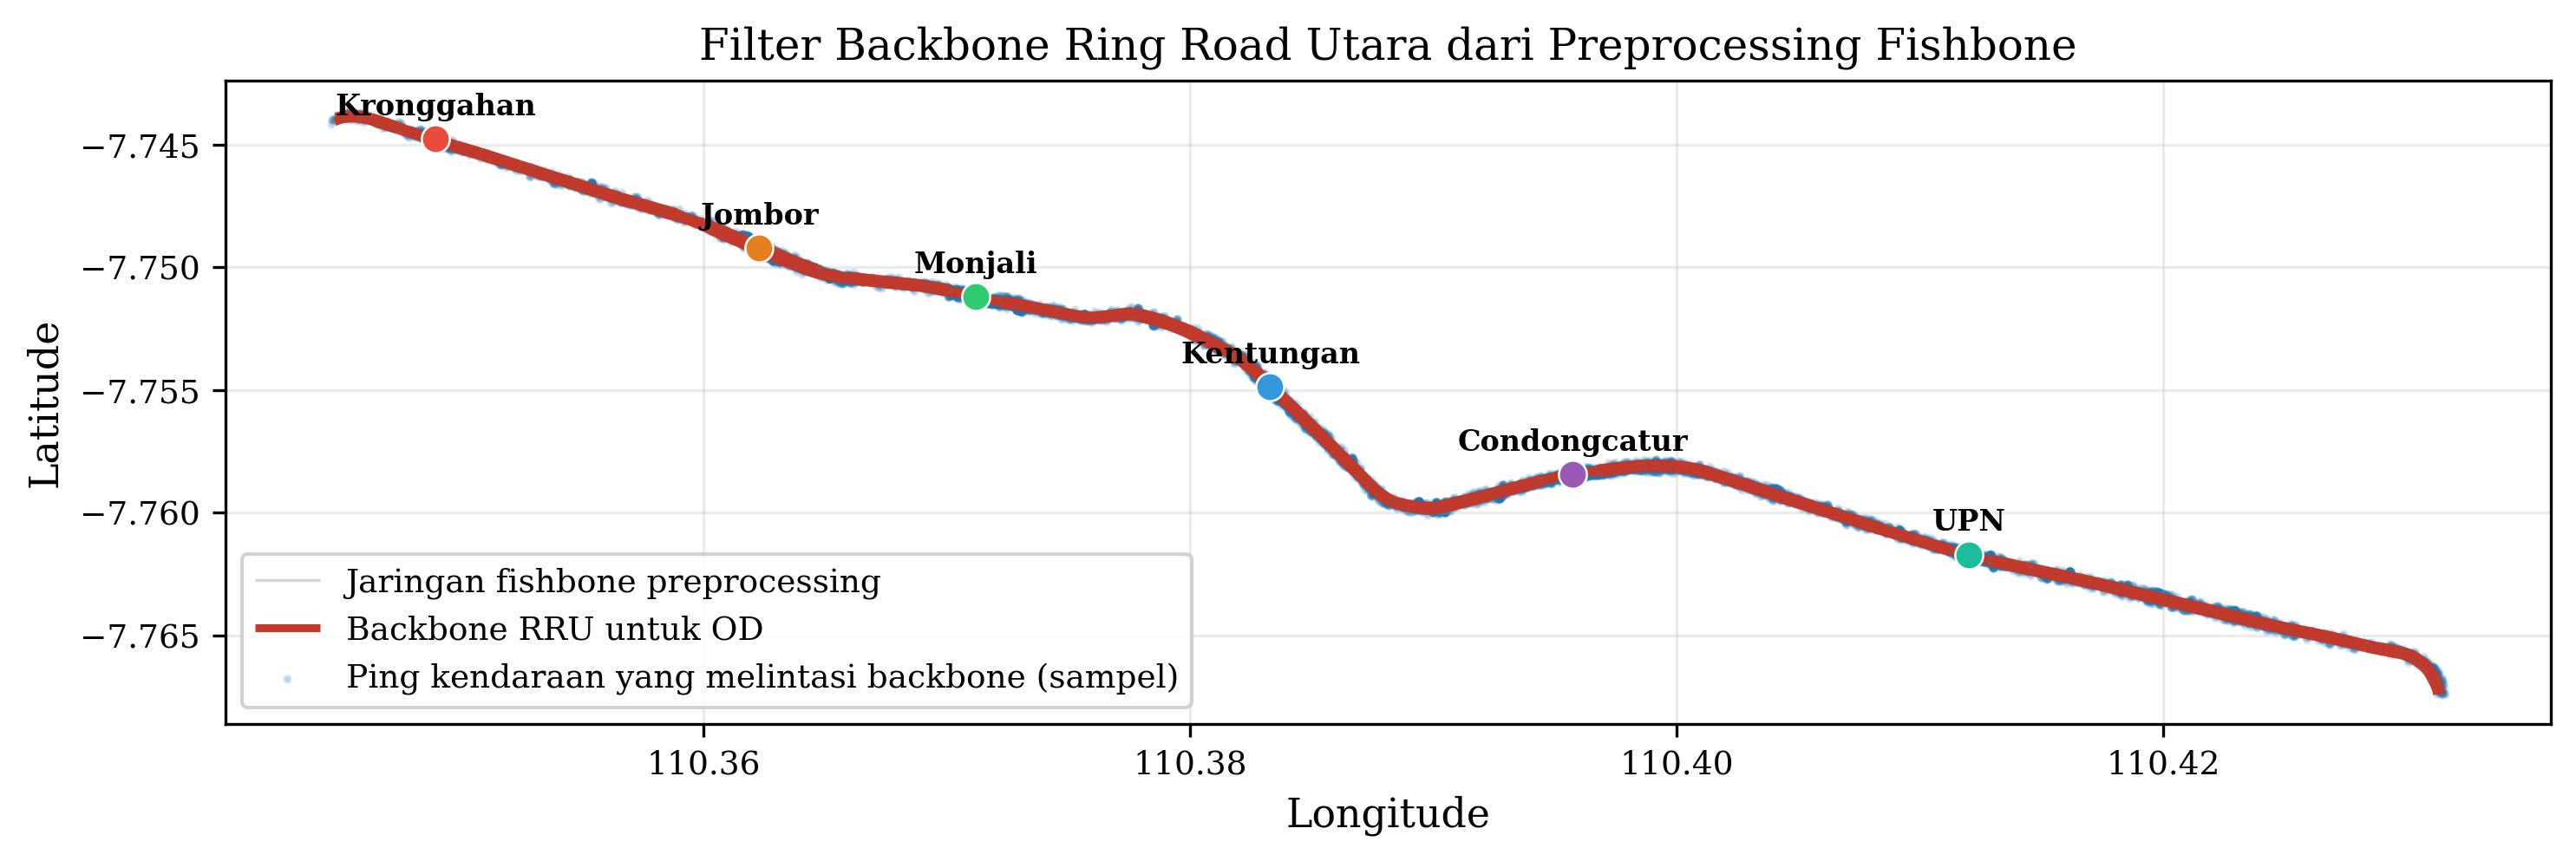
\includegraphics[width=0.95\textwidth]{../results/figures/network/rru_backbone_vehicle_map.png}
\caption{Jaringan RRU bersih dan sampel titik GPS kendaraan yang lolos praproses}
\label{fig:network-backbone}
\end{figure}

\section{Praproses Data}

Praproses data dilakukan untuk menyaring data wilayah kajian menjadi data kendaraan terindikasi pada koridor RRU. Ringkasan reduksi data pada setiap tahap ditunjukkan pada Tabel \ref{tab:reduksi}.

\begin{table}[htbp]
\centering
\caption{Reduksi Data pada Setiap Tahap Praproses}
\label{tab:reduksi}
\begin{tabular}{lrrr}
\hline
Tahap & Titik GPS & MAID Unik & Persentase Titik GPS\\
\hline
Data wilayah kajian (\texttt{output\_bbox}) & 15.386.869 & 370.778 & 100,0\%\\
R-tree candidates pada jaringan RRU & 839.304 & 45.691 & 5,5\%\\
\textit{Bilocation collapse} & 552.413 & 42.613 & 3,6\%\\
Klasifikasi moda kendaraan bermotor & 236.700 & 8.458 & 1,5\%\\
Trip valid hasil segmentasi & 212.407 & 8.382 & 1,4\%\\
\hline
\end{tabular}
\end{table}

\subsection{Bounding Box Filter}

Tahap pertama menggunakan data yang telah diekstraksi pada wilayah kajian Ring Road Utara. Data ini menjadi masukan awal untuk penyaringan spasial terhadap jaringan jalan, sehingga persentase reduksi pada Tabel \ref{tab:reduksi} dihitung terhadap \texttt{output\_bbox.parquet}.

\subsection{R-tree Edge Candidates}

Penyaringan spasial dilakukan menggunakan indeks R-tree. Setiap titik GPS dipasangkan dengan segmen jalan kandidat pada jaringan RRU dalam radius 20 meter. Titik yang tidak memiliki kandidat jalan dalam radius tersebut dieliminasi. Pemilihan toleransi spasial diperlukan karena data GPS aktif tetap mengandung galat posisi, terutama pada lingkungan perkotaan; studi akurasi A-GPS pada ponsel menunjukkan bahwa galat posisi dapat bervariasi dan tidak selalu berada tepat pada geometri jalan \cite{zandbergen2011}. Dalam konteks lokal, penelitian Nurlita (2024) juga menggunakan toleransi spasial pada pengolahan MPD aktif berbasis GPS \cite{nurlita2024}. Oleh karena itu, ambang 20 meter diperlakukan sebagai pilihan operasional yang konservatif untuk menyeimbangkan retensi titik dan risiko memasukkan titik dari jalan paralel atau area non-koridor.

Analisis sensitivitas ambang R-tree menunjukkan bahwa ambang 10 meter menghasilkan 694.708 kandidat titik setelah penghapusan MAID singleton, sedangkan ambang 20 meter menghasilkan 839.304 kandidat titik. Jika dibandingkan dengan 20 meter, ambang 10 meter menurunkan kandidat sekitar 17,2\%, sedangkan ambang 30 meter menaikkan kandidat sekitar 12,9\%. Pada ambang lebih besar, seperti 50 meter, jumlah kandidat meningkat sekitar 71,5\% dibandingkan 20 meter. Oleh karena itu, ambang 20 meter tidak diposisikan sebagai nilai optimal universal, tetapi sebagai kompromi konservatif untuk analisis koridor RRU.

\subsection{Bilocation Collapse}

Tahap \textit{bilocation collapse} menggabungkan titik-titik duplikat atau titik berdekatan yang muncul pada waktu yang sama dari mekanisme pencuplikan GPS. Tahap ini mengurangi artefak pengamatan ganda tanpa menambahkan titik sintetik baru.

\subsection{Klasifikasi Moda Transportasi}

Setelah \textit{bilocation collapse}, dilakukan klasifikasi moda transportasi berbasis fitur kecepatan untuk mempertahankan MAID yang menunjukkan indikasi kendaraan bermotor. Suatu MAID diklasifikasikan sebagai kendaraan bermotor apabila kecepatan maksimum antarping mencapai minimal 25 km/jam atau persentil ke-95 kecepatan mencapai minimal 15 km/jam. Ambang tersebut digunakan untuk mengurangi kontribusi pola yang cenderung stasioner atau berkecepatan rendah. Karena tidak tersedia label moda hasil survei lapangan, klasifikasi ini diperlakukan sebagai filter indikatif berbasis ambang, bukan klasifikasi moda yang tervalidasi pada tingkat individu.

\section{Map Matching}

\textit{Map matching} dilakukan menggunakan metode geometris \textit{nearest-edge} berdasarkan taksonomi Quddus et al. (2007) \cite{quddus2007}. Untuk setiap titik GPS yang memiliki kandidat R-tree, dipilih segmen jalan terdekat berdasarkan jarak geometris. Pada hasil pipeline terbaru, 236.700 titik GPS dicocokkan secara geometris ke jaringan RRU dengan rata-rata jarak 6,0 meter, median 5,0 meter, persentil ke-90 sebesar 12,4 meter, dan persentil ke-99 sebesar 19,2 meter. Statistik jarak tersebut merupakan statistik pasca-filter radius 20 meter, sehingga digunakan sebagai deskripsi kedekatan titik terhadap jaringan analisis dan bukan sebagai validasi independen akurasi \textit{map matching}.

Pemilihan metode geometris dibandingkan HMM didasarkan pada dua pertimbangan. Pertama, jaringan yang dianalisis merupakan koridor terbatas sehingga kompleksitas topologi relatif rendah. Kedua, data MPD aktif memiliki frekuensi pencuplikan yang tidak seragam dan banyak trip memiliki jumlah ping terbatas. Literatur \textit{map matching} untuk trajektori \textit{low-sampling-rate} menunjukkan bahwa jarak antarping yang besar meningkatkan ketidakpastian rute dan menurunkan kemampuan rekonstruksi lintasan detail \cite{lou2009,zheng2012,bian2020}. Dengan kondisi tersebut, rekonstruksi probabilistik yang rinci berisiko menghasilkan kepastian semu, sehingga penelitian ini memilih pendekatan geometris sederhana dan menempatkan hasilnya sebagai pencocokan indikatif terhadap jaringan analisis.

\section{Segmentasi Trajektori}

Setiap urutan ping per MAID disegmentasi menjadi unit perjalanan (trip) menggunakan metode berbasis gap waktu \cite{zheng2015}. Ambang batas yang digunakan adalah 10 menit atau 600 detik, mengikuti praktik pada penelitian sebelumnya dengan dataset sejenis \cite{nurlita2024}. Ambang 10 menit diperlakukan sebagai pilihan operasional, bukan batas universal. Trip valid didefinisikan sebagai segmen perjalanan yang memiliki minimal dua titik GPS.

Hasil segmentasi menghasilkan 38.973 trip valid dari 8.382 MAID. Median durasi trip adalah 223 detik, sedangkan rata-rata durasi trip adalah 333 detik. Median jumlah ping per trip adalah 4 ping, dengan rata-rata 5,45 ping per trip. Sebanyak 70,37\% trip memiliki paling banyak 5 ping, sedangkan hanya 12,88\% trip memiliki sedikitnya 10 ping. Distribusi ini menunjukkan bahwa data bersifat sparse, sehingga analisis diarahkan pada pola agregat dan bukan rekonstruksi lintasan detail.

\section{Pelabelan Persimpangan}

Setiap titik GPS yang telah di-\textit{map match} dilabeli berdasarkan kedekatan terhadap enam persimpangan utama. Zona persimpangan didefinisikan sebagai lingkaran dengan radius 200 meter dari titik pusat persimpangan. Untuk setiap trip, origin didefinisikan sebagai persimpangan pertama yang terdeteksi dalam urutan trip, sedangkan destination didefinisikan sebagai persimpangan terakhir yang terdeteksi. Dengan definisi ini, OD yang dihasilkan merupakan OD zona teramati pada koridor RRU, bukan asal dan tujuan perjalanan sebenarnya di luar koridor. Radius 200 meter digunakan sebagai definisi operasional zona simpang; perubahan radius dapat memengaruhi jumlah ping dalam zona, jumlah trip dengan OD teridentifikasi, dan besarnya diagonal OD.

Dari 212.407 ping dalam trip valid, sebanyak 86.042 ping atau 40,5\% berada dalam zona persimpangan. Pelabelan OD menghasilkan 28.767 trip dengan origin dan destination yang teridentifikasi dari total 38.973 trip valid.

\section{Modul Analisis}

\subsection{Matriks Origin-Destination}

Matriks OD berukuran 6×6 dibangun dari pasangan origin dan destination setiap trip. Matriks dihitung untuk agregat keseluruhan, hari kerja vs akhir pekan, jam sibuk vs non-sibuk, per jam, dan per bulan. Jam sibuk didefinisikan sebagai pukul 07.00--09.00 dan 16.00--18.00 WIB.

\subsection{Indikator Intensitas Persimpangan}

Indikator intensitas persimpangan dihitung dari jumlah MAID unik dan jumlah ping yang teramati dalam zona persimpangan. Perhitungan dilakukan pada resolusi 15 menit, per jam, harian, bulanan, serta perbandingan hari kerja dan akhir pekan. Nilai ini tidak ditafsirkan sebagai volume lalu lintas aktual, tetapi sebagai intensitas pengamatan kendaraan dalam dataset MPD aktif.

\subsection{Klasifikasi Pola OD Zona Eksploratif}

Pola OD zona diklasifikasikan secara eksploratif berdasarkan pasangan zona asal dan tujuan trip. Kategori yang digunakan meliputi O=D atau zona sama, indikasi kedatangan dari arah barat/timur, dan indikasi keberangkatan menuju barat/timur. Karena sebagian besar trip hanya memiliki sedikit ping, hasil ini diposisikan sebagai indikasi pola pergerakan zona, bukan klasifikasi belokan aktual yang tervalidasi secara geometris.

\subsection{Analisis yang Tidak Dilakukan}

Penelitian ini tidak melakukan analisis \textit{catchment area} atau estimasi lokasi rumah pengguna. Keputusan ini diambil untuk menjaga fokus penelitian pada karakteristik pergerakan yang benar-benar teramati pada koridor RRU. Selain itu, estimasi lokasi rumah membutuhkan asumsi tambahan terhadap riwayat lokasi pengguna di luar koridor, sehingga berpotensi memperluas cakupan penelitian di luar tujuan utama penyusunan \textit{baseline} spatiotemporal koridor.
